%-----------------------------------------------------------------------------%
chapter{\babDua}
%-----------------------------------------------------------------------------%
Bagian ini menjelaskan teori-teori yang digunakan dalam penelitian. Teori yang dimaksud adalah pengetahuan yang terkait dengan pelaksanaan penelitian.

%-----------------------------------------------------------------------------%
\section{Deep Learning}
%-----------------------------------------------------------------------------%
\deeplearning merupakan algoritma \ml yang memanfaatkan arsitektur \nn. Cara kerja arsitektur ini terinspirasi oleh struktur otak manusia yang tersusun dari neuron-neuron. Berbeda dengan Artificial Neural Network biasa, Neural Network pada Deep Learning memiliki struktur yang lebih kompleks, terdiri dari lebih dari satu hidden layer. Ide utama dari Deep Learning adalah bagaimana komputer dapat belajar dari pengalaman dengan cara melatih \nn menggunakan data-data yang berjumlah besar. \deeplearning merupakan salah satu contoh dari \textit{Supervised Learning} yang berarti \nn dilatih menggunakan data yang telah diketahui labelnya. \nn yang telah dilatih dapat digunakan untuk menentukan label atau skor dari data-data baru \cite{deeplearning2}. 

Deep Learning dikenal memiliki akurasi yang lebih tinggi dibandingkan algoritma Machine Learning konvensional karena kompeksitas Neural network yang digunakan. Akurasi dari prediksi/inference bergantung pada jenis arsitektur \nn, kualitas dan kuantitas data yang digunakan untuk melatih, serta jenis permasalahan yang diselesaikan. Pada Deep Learning terdapat berbagai jenis arsitektur. Tiga arsitektur yang populer adalah Deep Neural Network, Convolutional Neural Network, dan Recurrent Neural Network. Deep Neural Network. Masing-masing arsitektur memiliki kelebihan dan kekurangan masing-masing. Untuk setiap permasalahan perlu dipilih arsitektur yang tepat agar mendapatkan akurasi maksimal.

Deep Neural Network (DNN) merupakan jenis arsitektur Deep Learning yang paling sederhana. DNN merupakan \nn yang terdiri dari satu input layer, satu atau lebih hidden layer, dan satu output layer. Layer-layer pada arsitektur ini merupakan fully connected layer. Setiap layer tersusun dari node-node yang masing-masing terhubung dengan semua node dari layer-layer tetangganya. Nilai dari suatu node pada layer ke-l merupakan hasil penerapan suatu activation function terhadap perkalian dari node-node pada layer ke-(l-1) dengan weight parameter tertentu \cite{deeplearningmatrix}. \pic~\ref{fig:dnn} menunjukkan contoh arsitektur DNN.

\begin{figure}
	\centering
	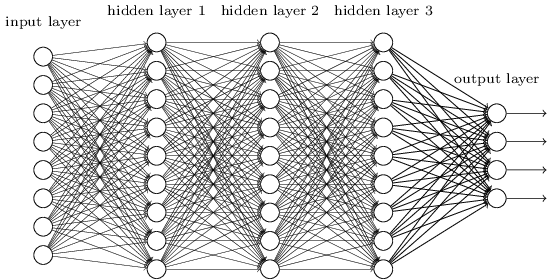
\includegraphics[width=0.50\textwidth]
	{pics/dnn.png}
	\caption{Contoh Arsitektur Deep Neural Network.}
	\label{fig:dnn}
\end{figure}

Karena arsitekturnya yang sederhana, DNN pada banyak kasus memiliki performa yang tidak sebaik arsitektur lain seperti CNN atau RNN. DNN lebih tepat digunakan untuk melakukan tugas-tugas prediksi sederhana. Fitur-fitur dari data harus sudah ditentukan terlebih dahulu apabila ingin melakukan training dan inference pada DNN. Beban komputasi DNN lebih ringan dari arsitektur lain seperti CNN.

Convolutional Neural Network (CNN) merupakan arsitektur \deeplearning yang sering digunakan dalam bidang pengolahan citra. CNN pada umumnya terdiri dari beberapa convolution layer, pooling layer, dan fully-connected layer. Convolution layer dan Pooling layer merupakan jenis layer pada CNN yang tidak terdapat pada arsitektur-arsitektur lain. Convolution layer biasanya berfungsi untuk mengekstrak fitur-fitur dari data yang akan diprediksi secara otomatis. Pada DNN fitur-fitur dari data harus ditentukan sendiri secara manual. Pada convolution layer terjadi operasi konvolusi terhadap input menggunakan suatu kernel tertentu. Pooling layer berfungsi untuk mereduksi ukuran data dengan cara melakukan sampling. Data yang direduksi biasanya adalah keluaran dari convolution layer \cite{deeplearningmatrix}. Fully-connected layer biasanya diletakkan pada bagian akhir arsitektur CNN. layer ini berfungsi untuk melakukan prediksi, sama seperti DNN, dengan menggunakan fitur-fitur hasil ekstraksi convolution layer. \pic~\ref{fig:cnn} merupakan contoh arsitektur CNN.

\begin{figure}
	\centering
	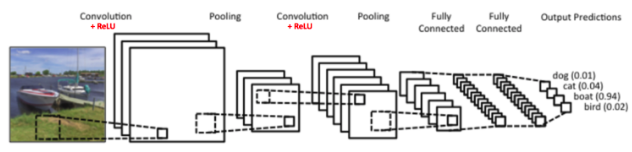
\includegraphics[width=0.50\textwidth]
	{pics/cnn.png}
	\caption{Contoh Arsitektur \conv \nn.}
	\label{fig:cnn}
\end{figure}

Recurrent Neural Network (RNN) merupakan arsitektur Deep Learning yang dapat digunakan untuk jenis data yang bersifat sekuensial. Arsitektur ini terdiri dari input layer, hidden layer, dan output layer yang mengandung loop. Hasil prediksi dari output layer pada suatu waktu \textit{t} digunakan untuk mengubah parameter dari layer-layer sebelumnya untuk melakukan prediksi pada waktu \textit{t+1}. Jadi dapat dikatakan bahwa output dari suatu layer pada suatu waktu bergantung pada output dari layer itu sendiri pada waktu-waktu sebelumnya \cite{deeplearning2}. \pic~\ref{fig:rnn} merupakan contoh arsitektur RNN.

\begin{figure}
	\centering
	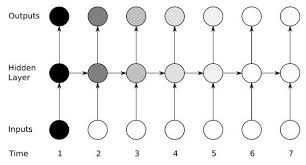
\includegraphics[width=0.50\textwidth]
	{pics/rnn.jpeg}
	\caption{Contoh Arsitektur Recurrent Neural Netowork.}
	\label{fig:rnn}
\end{figure}

RNN sering digunakan dalam bidang Natural Language Processing (NLP) karena tugas-tugas pada NLP pada umumnya melibatkan  pengolahan teks atau suara dengan aturan bahasa, sehingga datanya bersifat sekuensial. 

Dengan melihat contoh-contoh arsitektur \deeplearning di atas, dapat diketahui bahwa Deep Learning memiliki beban komputasi yang cukup besar, terutama pada CNN, karena melibatkan banyak parameter dan banyak layer. Oleh karena itu, penggunaan CPU saja dirasa kurang cukup dalam menjalankan operasi-operasi pada Deep Learning.
%-----------------------------------------------------------------------------%
\section{Deep Learning Training dan Inference}
%-----------------------------------------------------------------------------%
Sama seperti \nn biasa, arsitektur \nn dalam Deep Learning memiliki parameter \weight pada setiap layer yang digunakan untuk menghitung skor dari input pada suatu \layer dan meneruskannya ke \layer berikutnya. Deep Learning terdiri dari dua  tahap yaitu training dan inference. Pada tahap training, model \nn dilatih menggunakan sekumpulan data. Dalam proses ini weight parameter terus-menerus memperbarui nilainya hingga pada akhirnya konvergen. Nilai parameter yang konvergen menandakan weight tersebut telah merepresentasikan data-data training \cite{deeplearningmatrix}.

Untuk mengawali proses \training, \weight awal diberikan terlebih dahulu kepada model. Biasanya \weight awal ini merupakan angka-angka acak berdasarkan suatu distribusi tertentu. Selanjutnya, model dengan \weight awal yang belum tersebut digunakan untuk melakukan prediksi label atau skor dari data-data training dengan cara melakukan \textit{forward pass} di sepanjang model, mulai dari \layer pertama (input \layer) hingga mencapai \layer terakhir (\outputa \layer). Hasil prediksi pada output layer kemudian dibandingkan dengan label aslinya. Nilai \error dari prediksi dapat dihitung menggunakan fungsi error tertentu, misalnya \textit{Mean Square Error}. Informasi \error ini kemudian dikirim kembali ke \layer-\layer sebelumnya dan akan digunakan oleh \layer-\layer terebut untuk memperbarui parameter \weight. \textit{Weight} dapat diperbarui menggunakan algoritma atau fungsi pembaruan \weight tertentu. Proses mengembalikan \error ke belakang ini disebut \textit{back propagation} \cite{trainvsinfer}. 

Setelah \training selesai, model \nn dapat digunakan untuk melakukan proses \inference. Tahap \inference merupakan tahap dimana model yang telah dilatih digunakan untuk melakukan prediksi. Proses prediksi ini sama seperti prediksi ketika melakukan \training, yaitu dengan melakukan \textit{forward-pass} terhadap input data mulai dari \inputa \layer hingga \outputa \layer pada model. Letak perbedaan proses \inference dan \training adalah pada tahap \textit{back-propagation}. Setelah melakukan prediksi pada proses \inference, tidak lagi dilakukan \textit{back-propagation} terhadap \error hasil prediksi seperti pada proses \training. Tujuan dari \inference adalah hanyalah mendapatkan hasil prediksi skor atau label yang dikeluarkan oleh model yang telah dilatih \cite{trainvsinfer}. 

\pic~\ref{fig:trainvsinfer} menunjukkan perbedaan proses \training dan \inference pada Deep Learning. Terlihat bahwa pada tahap \training terjadi pemrosesan data pada dua arah (forward-pass dan back-propagation), sedangkan pada \inference hanya terjadi satu arah (forward-pass saja).

\begin{figure}
	\centering
	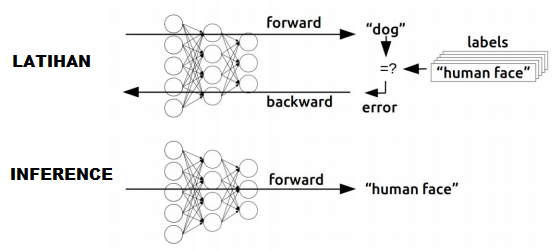
\includegraphics[width=0.50\textwidth]
	{pics/trainingvsinference.png}
	\caption{Perbedaan proses \training dan \inference pada \deeplearning.}
	\label{fig:trainvsinfer}
\end{figure}

\section{Operasi-operasi Deep Learning Inference}
%-----------------------------------------------------------------------------%
Tahap inference pada Deep Learning melibatakan banyak operasi matriks. Matriks yang dioperasikan biasanya adalah input data dan weight atau kernel pada suatu layer. Perkalian matriks-vector dan konvolusi merupakan dua operasi pada Deep Learning Inference yang memiliki kompleksitas tinggi. Berikut adalah penjelasan lebih lanjut mengenai dua operasi tersebut.

\subsection{Perkalian Matriks-Vector}
Operasi perkalian matriks-vector pada Deep Learning inference merupakan salah satu operasi yang memiliki beban komputasi terbesar. Perkalian matriks-vector dapat terjadi pada fully-connected layer. Pada layer ke-\textit{l}, parameter \textit{weight} disimpan dalam bentuk matriks yang berukuran \textit{MxN} dimana \textit{M} adalah banyaknya node pada layer ke-l dan \textit{N} adalah banyaknya node pada layer ke-(l-1) \cite{deeplearningmatrix}. Baris ke-i pada \textit{weight} matriks dari layer ke-l tersebut merupakan weight dari node ke-i pada layer ke-l. Untuk memperoleh nilai node-node pada layer ke-l, matrix \textit{MxN} tersebut dikalikan dengan vector sepanjang \textit{N} yang berisi nilai-nilai node pada layer ke-(l-1). Hasilnya adalah vector sepanjang \textit{M}. Jika ada, bias ditambahkan kepada vector tersebut. Selanjutnya, activation function diterapkan terhadap setiap elemen vector sehingga menghasilkan vector sepanjang \textit{M} yang merupakan nilai node-node pada layer ke-l. \pic~\ref{fig:fcmatmul} adalah ilustrasi dari operasi perkalian matriks-vector pada fully-connected layer.

\begin{figure}
	\centering
	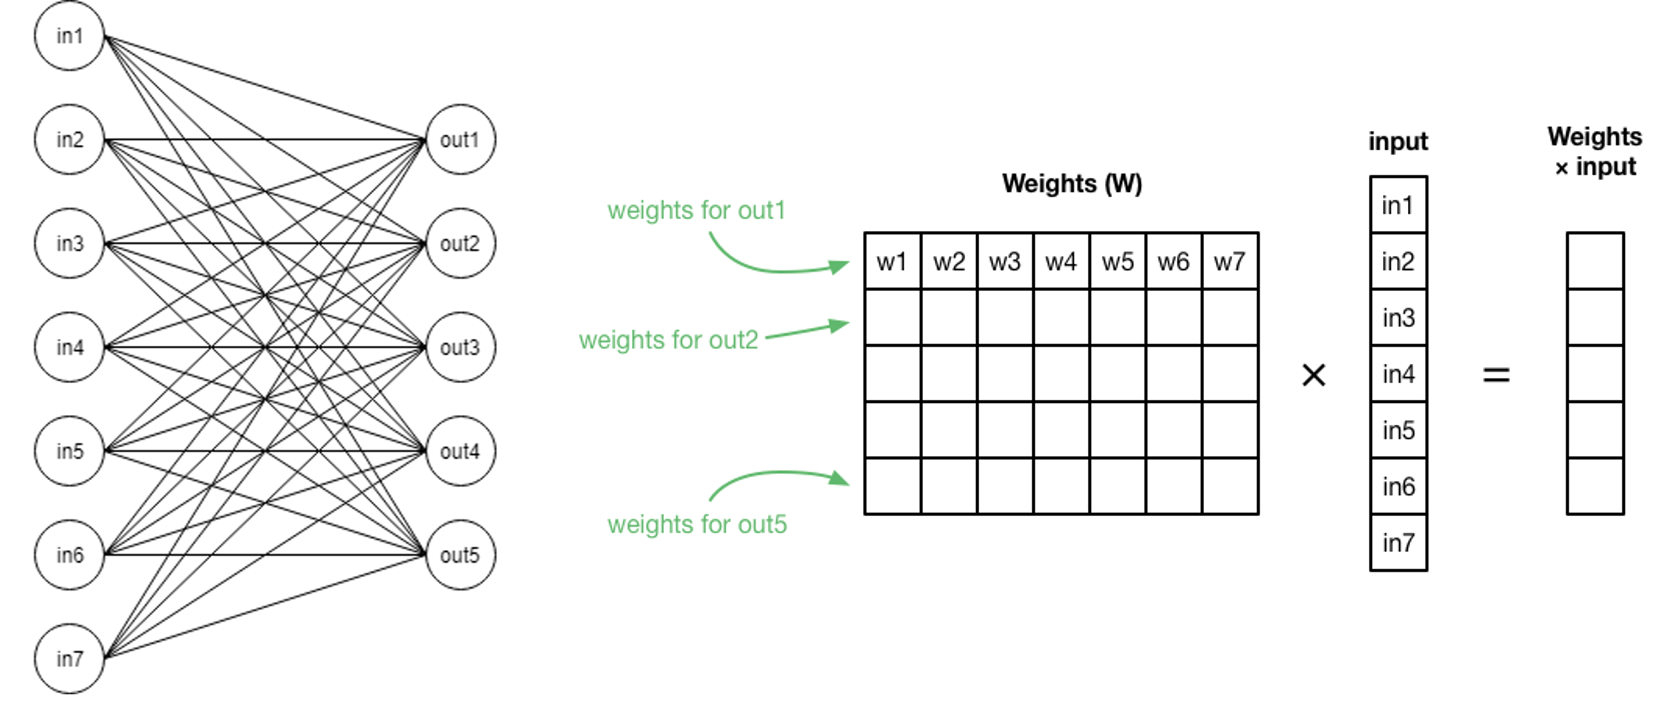
\includegraphics[width=0.50\textwidth]
	{pics/fcmatmul.png}
	\caption{Ilustrasi perkalian matriks dengan vector pada fully-connected layer saat mengalikan weight dengan input.}
	\label{fig:fcmatmul}
\end{figure}

Misalkan matrix weight untuk layer ke-l adalah \textit{Mat} dan vector input dari layer ke-(l-1) adalah \textit{Vec}, kompleksitas dari operasi perkalian matriks pada layer ke-l dapat dihitung sebagai berikut.

\noindent \begin{align}\label{eq:mamulcomplexity} \nonumber
	dot(Mat[row=1], Vec[col=1]) &= O(N) \\ \nonumber
	dot(Mat[row=2], Vec[col=1]) &= O(N) \\ \nonumber
	.\\ \nonumber
	.\\ \nonumber
	.\\ \nonumber
	dot(Mat[row=M], Vec[col=1]) &= O(N) \\ 
	\cline{1-2}
	\nonumber Total kompelksitas &= M*O(N) \\ 
	 &= O(MN)
\end{align} 

\subsection{Konvolusi Matriks}
Operasi konvolusi terjadi pada convolution layer dari CNN. Konvolusi merupakan penerapan filter/kernel terhadap input dengan mengkonvolusikan kernel tersebut \cite{deeplearningmatrix}. Proses konvolusi dapat menggunakan satu atau lebih filter. Input, output, dan filter pada convolution layer masing-masing merupakan matriks 3 dimensi yang merepresentasikan lebar, tinggi, dan kedalaman (channel). Ukuran dari input, filter, dan output pada convolution layer memilliki beberapa aturan sebagai berikut. 

\begin{enumerate}
\item Tinggi dan lebar filter selalu lebih kecil atau sama dengan tinggi dan lebar intput.
\item Kedalaman input selalu sama dengan kedalaman filter.
\item Banyaknya filter sama dengan kedalaman output.
\item Tinggi dan lebar output selalu lebih kecil atau sama dengan tinggi dan lebar intput.
\end{enumerate}	

Pada proses konvolusi, posisi filter dimulai dari ujung kiri atas dari input. Filter kemudian bergeser ke kanan dan kebawah dengan stride (jarak geser) yang ditentukan. Pada suatu posisi filter, masing-masing elemen pada filter dikalikan dengan elemen-elemen matriks input yang bersesuaian dengan posisi filter tersebut (seperti dot product pada vector). Hasil dari satu kali operasi tersebut merupakan satu elemen dari matriks output pada posisi yang bersesuaian.  Sehingga, setelah proses konvolusi selesai untuk satu filter, akan terbentuk satu lapis output dua dimensi. Jika semua filter sudah diterapkan, maka akan terbentuk output tiga dimensi dengan kedalaman sesuai dengan banyaknya filter. \pic~\ref{fig:conv} menunjukkan contoh operasi konvolusi dengan input berukuran 5x5x1, filter berukuran 3x3x1, dan nilai stride 1.

\begin{figure}
	\centering
	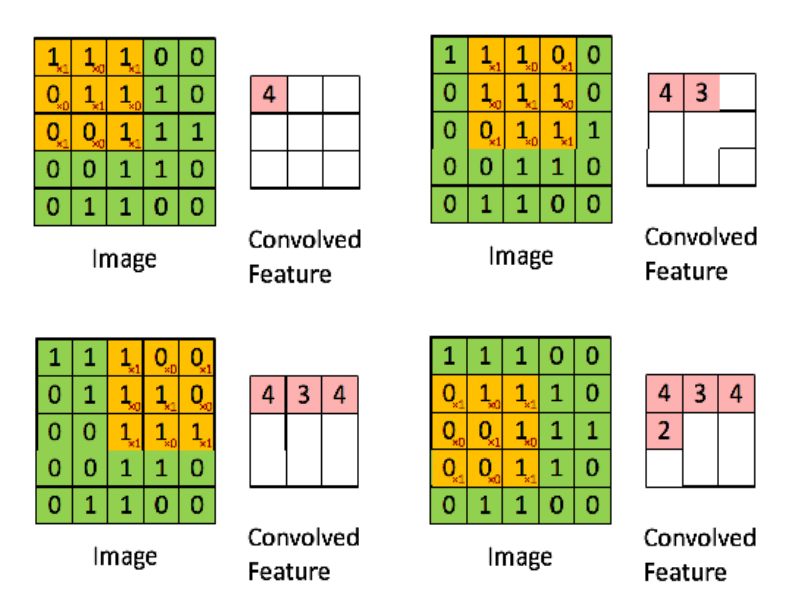
\includegraphics[width=0.50\textwidth]
	{pics/conv.png}
	\caption{Contoh Operasi Konvolusi. Image merupakan gambar masukan, convolved feature merupakan keluaran dari konvolusi.}
	\label{fig:conv}
\end{figure}

Pada operasi konvolusi dengan input berukuran MxNxD, filter berukuran M'xN'xD, banyak filter adalah K, kompleksitas dapat dihitung sebagai berikut. Pada suatu posisi filter, kompleksitas dot product untuk menghasilkan satu elemen output adalah sebagai berikut.

\noindent \begin{align}\label{eq:dotcomplexity} Kompleksitas dot product = O(M'N'D) \end{align}

\noindent Kernel bergeser sebanyak O(N) ke kanan dikalikan dengan sebanyak O(M) ke bawah. Diperoleh komleksitas geser sebagai berikut.

\noindent \begin{align}\label{eq:gesercomplexity} Kompleksitas geser kernel = O(MN) \end{align} 

\noindent Menggunakan \equ~\ref{eq:dotcomplexity} dan \equ~\ref{eq:gesercomplexity}, diperoleh total kompleksitas sebagai berkut.

\noindent \begin{align}\label{eq:convcomplexity} \nonumber Total ompleksitas &= kompleksitas dot product * kompleksitas geser kernel \\ &= O(MM'NN'DK) \end{align}

\noindent Dengan kompleksitas \textit{O(MM'NN'DK)}, konvolusi merupakan operasi paling mahal jika dibandingkan operasi pada layer-layer lain. 

\section{Tensorflow}
%-----------------------------------------------------------------------------%
Tensorflow merupakan perangkat lunak \textit{open-source} yang digunakan untuk komputasi numerik menggunakan representasi graf yang membentuk serangkaian operasi \cite{tensorflow}. Node pada graf merepresentasikan suatu operasi sedangkan edge mereperesentasikan tensor atau multidimensional array yang merupakan input atau output dari suatu operasi. Tensorflow dikembangkan oleh Google untuk mendukung penelitian pada bidang \ml dan Deep Learning. Salah satu fitur menarik dari Tensorflow adalah adanya dukungan untuk Deep Learning inference pada perangkat \textit{mobile} melalui \textit{library} Tensorflow Mobile dan Tensorflow Lite. Tensorflow dan Tensorflow Lite diimplementasikan menggunakan bahasa C/C++ dengan menyediakan API dalam bahasa C++, Python, dan Java.

\section{Tensorflow Lite}
%-----------------------------------------------------------------------------%
Tensorflow Lite merupakan salah satu library dari Tensorflow yang dapat digunakan untuk \deeplearning \inference pada perangkat mobile \cite{tflite}. Selain Tensorflow Lite, terdapat library sejenis yaitu Tensorflow Mobile. Tensorflow Lite, yang dirilis pada November 14, 2017, merupakan versi perbaikan dari Tensorflow Mobile yang telah dirilis terlebih dahulu. Tensorflow Lite mendukung penggunaan CNN, DNN, dan RNN sebagai model Neural Network. 

Untuk menjalankan inference, Tensorflow Lite menggunakan model Neural Network yang telah dilatih dan direpresentasikan dalam file dengan ekstensi .tflite. File ini sebenarnya merupakan graf komputasi yang berisi serangkaian node (operation) dan edge (tensor). Model file tersebut dimuat oleh C++ API untuk kemudian diteruskan ke interpreter. Interpreter mengeksekusi model menggunakan serangkaian kernel yang dimuat secara selektif (hanya kernel terkait saja yang dimuat). \pic~\ref{fig:tflite} merupakan ilustrasi dari arsitektur Tensorfow Lite.

\begin{figure}
	\centering
	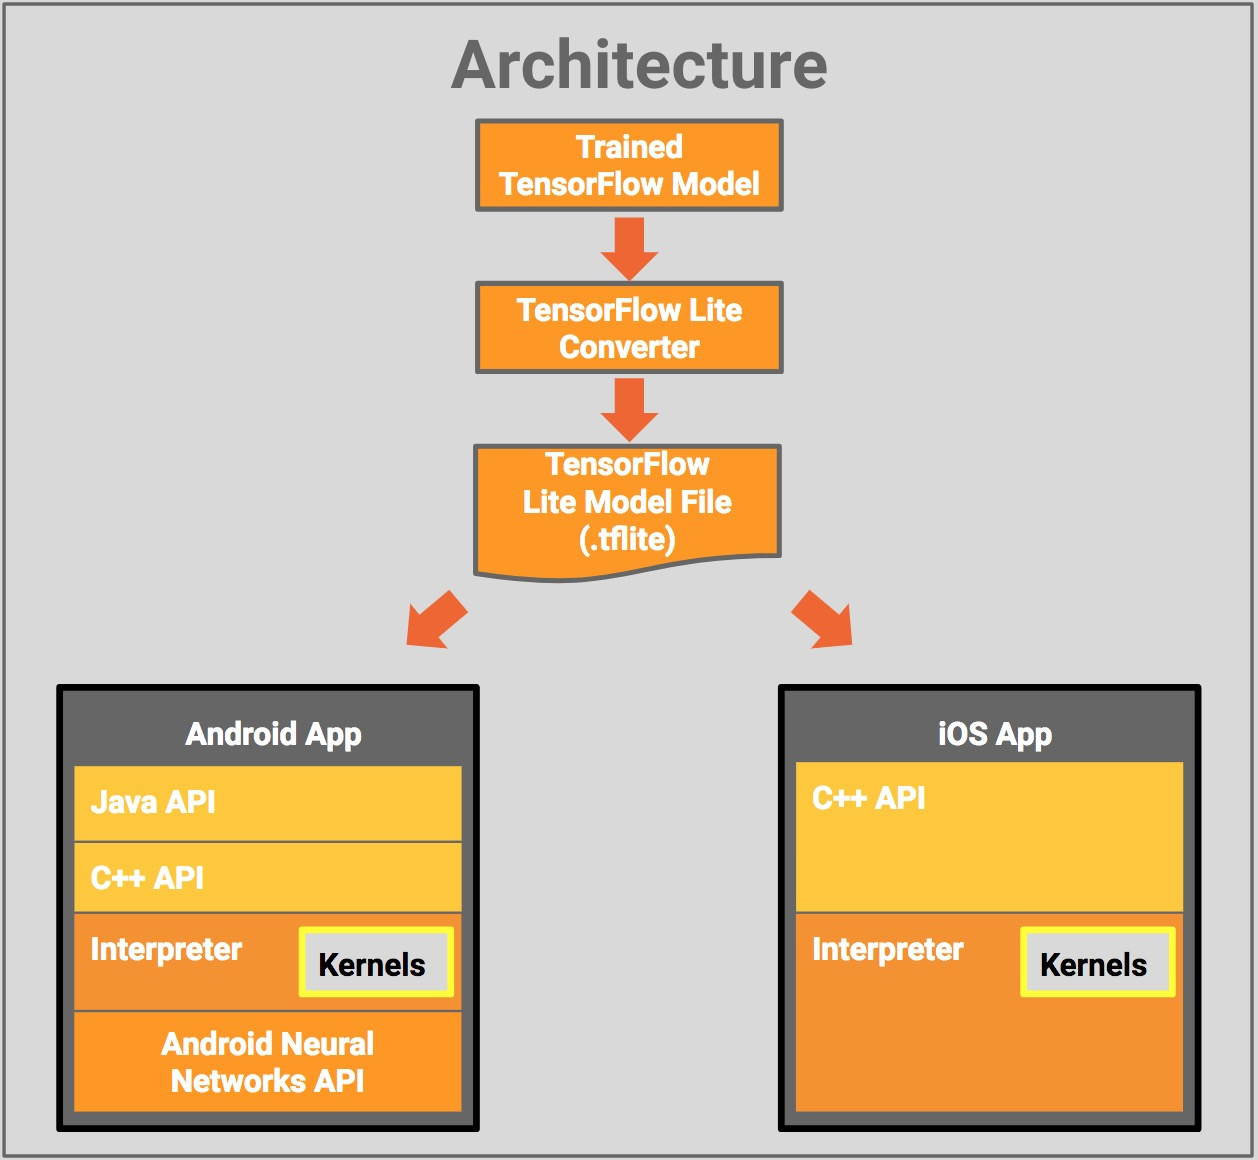
\includegraphics[width=0.50\textwidth]
	{pics/tflite.jpg}
	\caption{Ilustrasi dari arsitektur Tensorflow Lite.}
	\label{fig:tflite}
\end{figure}

Berbeda dengan Tensorflow Mobile, Tensorflow memiliki kernel tersendiri yang berisi operasi-operasi \deeplearning \inference dan terpisah dari core Tensorflow. Sehingga, modifikasi kernel Tensorflow Lite dengan menambahkan program OpenCL atau Vulkan  tidak akan mengubah perilaku dari program utama Tensorflow.

Dibandingkan dengan Tensorflow Mobile, Tensorflow Lite telah mendapatkan berbagai macam optimisasi.Performa inference yang dihasilkan lebih baik daripada Tensorflow Mobile. Beberapa bug pada Tensorflow Mobile juga telah diperbaiki pada Tensorlfow Lite. Selain itu, fitur-fitur yang ditawarkan Tensorflow Lite juga lebih banyak dibandingkan Tensorflow Mobile. Berikut adalah beberapa keunggulan Tensorflow Lite dibandingkan Tensorflow Mobile \cite{tflite}.

\begin{enumerate}
	\item Memiliki fitur yang dapat memprune node dari operation graph yang tidak terpakai pada proses inference.
	\item Memiliki kernel yang mendukung komputasi dalam 8-bit fixed point.
	\item Optimasi performa untuk operasi floating point maupun fixed point.
	\item Menggunakan pre-fused activation pada model Deep Learning.
	\item Memuat kernel secara selektif sehingga menghemat memori.
\end{enumerate}

\section{OpenCL}
%-----------------------------------------------------------------------------%
OpenCL merupakan API untuk pemrograman paralel dengan memanfaatkan prosesor yang berbeda-beda seperti CPU, GPU, DSP, dan FPGA, sehingga dapat meningkatkan performa komputasi secara signifikan \cite{opencl}. Pada OpenCL terdapat dua sisi program, yaitu host dan device. Device adalah prosesor target, sedangkan host adalah yang mengatur jalannya program pada device. Tugas yang dilakukan oleh host antara lain mencari device, menginisialisasi konteks, mengkompilasi kernel, menyalin data dari host ke device memory, menjalankan kernel, dan mengambil data hasil komputasi dari device memory. Program host ditulis dalam bahasa C++ dengan ekstensi OpenCL. \pic~\ref{fig:hostdevice} mengilustrasikan bagaimana host mengatur komputasi pada device.

\begin{figure}
	\centering
	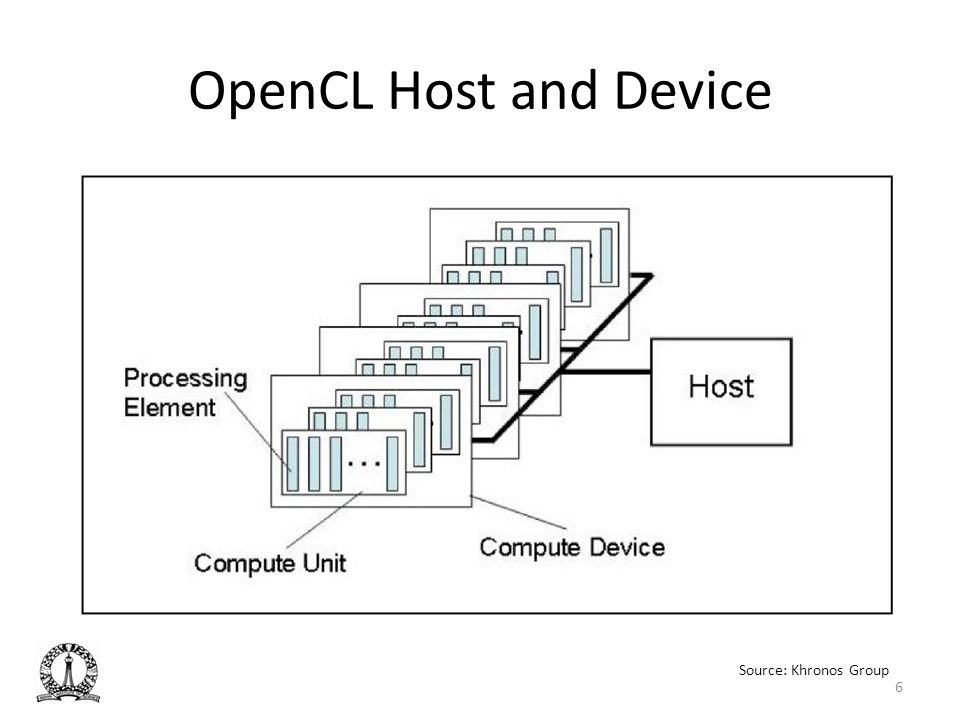
\includegraphics[width=0.50\textwidth]
	{pics/openclhostdevice.jpg}
	\caption{Host mengatur jalannya komputasi pada satu atau lebih device.}
	\label{fig:hostdevice}
\end{figure}

Program yang dijalankan pada device merupakan sekumpulan OpenCL kernel. Kernel ditulis menggunakan bahasa C dengan ekstensi OpenCL. Pada bagian host, kernel ditulis sebagai string dan dikompilasi terlebih dahulu sebelum dapat dieksekusi. Beberapa hal yang perlu dilakukan host sebelum menjalankan kernel pada OpenCL device adalah sebagai berikut.

\begin{enumerate}
	\item Membuat context. Context adalah environment dimana kernel dieksekusi. Pada context didefiniskan kernel yang digunakan, device yang digunakan, buffer/memory yang dapat diakses oleh device, properti dari memori tersebut, dan satu atau lebih command-queue untuk penjadwalan eksekusi kernel.
	\item Mempersiapkan kernel. Kernel adalah serangkaian instruksi yang dijalankan pada device. Kernel ditulis sebagai string dan dikompilasi menggunakan fungsi clBuildKernel() dari OpenCL API.
	\item Mempersiapkan buffer. Buffer object merupakan memory object yang menyimpan koleksi data secara linear dalam bytes. Buffer object dapat diakses menggunakan pointer pada kernel yang berjalan pada device. Konten dari buffer juga dapat dimanipulasi melalui host.
	\item Membuat command-queue. Command-queue merupakan objek yang menampung perintah-perintah yang akan dieksekusi pada device. Suatu command-queue dibuat unutk device yang spesifik dalam sebuah konteks.
\end{enumerate}

Kernel dapat disubmit ke command-queue dengan mendefinisikan banyaknya work-item dan work-group yang megeksekusi kernel. \pic~\ref{fig:context} mengilustrasikan bagaimana OpenCL kernel dieksekusi pada device.

\begin{figure}
	\centering
	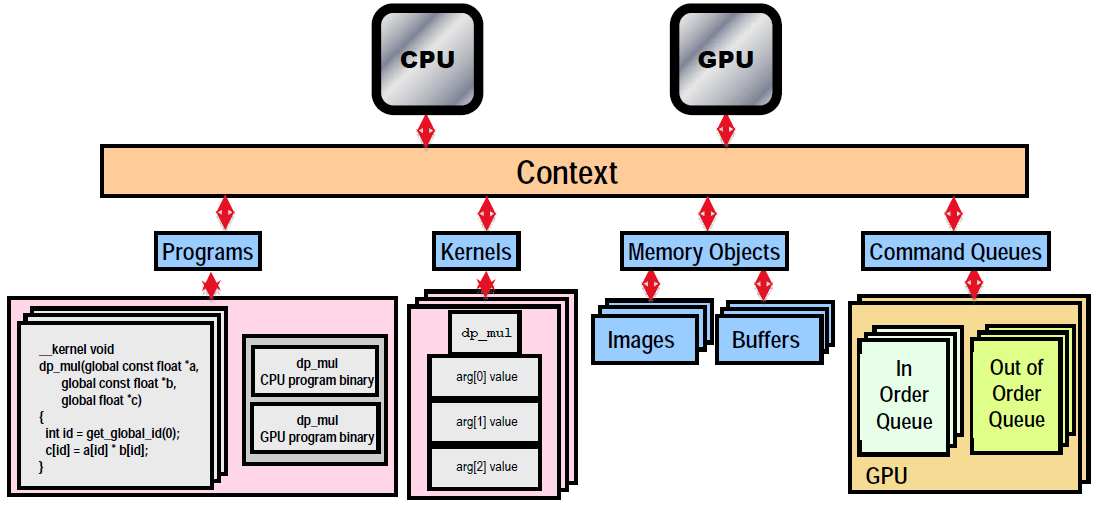
\includegraphics[width=0.50\textwidth]
	{pics/opencl-context.png}
	\caption{Cara kerja OpenCL.}
	\label{fig:context}
\end{figure}

OpenCL program dapat berjalan pada perangkat yang memiliki dukungan library OpenCL (libOpenCl.so). Pada NVidia GPU, library dapat diperoleh dalam paket installasi CUDA. Sedangkan pada perangkat android, beberapa vendor GPU seperti Adreno dan Mali menyertakan library OpenCL pada perangkat mereka. Library libOpenCl.so biasanya terletak pada direktori /system/vendor/lib/ dan dapat diambil melalui perintah adb pull pada Linux. Berikut adalah contoh program host dan device (kernel) pada OpenCL.

\begin{lstlisting}[frame=single]
/* OpenCL Host Example */
void clHello() {
    cl_device_id device_id = NULL;
    cl_context context = NULL;
    cl_command_queue command_queue = NULL;
    cl_mem memobj = NULL;
    cl_program program = NULL;
    cl_kernel kernel = NULL;
    cl_platform_id platform_id = NULL;
    cl_uint ret_num_devices;
    cl_uint ret_num_platforms;
    cl_int ret;

    char string[MEM_SIZE];

    /* Get Platform and Device Info */
    ret = clGetPlatformIDs(1, &platform_id, 
    &ret_num_platforms);
    ret = clGetDeviceIDs( platform_id, 
    CL_DEVICE_TYPE_DEFAULT, 1, &device_id, 
    &ret_num_devices);

    /* Create OpenCL context */
    context = clCreateContext( NULL, 1, &device_id, 
    NULL, NULL, &ret);

    /* Create Command Queue */
    command_queue = clCreateCommandQueue(context, 
    device_id, 0, &ret);

    /* Create Memory Buffer */
    memobj = clCreateBuffer(context, 
    CL_MEM_READ_WRITE,MEM_SIZE * sizeof(char), NULL, 
    &ret);

    /* Create Kernel Program from the source */
    program = clCreateProgramWithSource(context, 1, 
    (const char **)&CLCL_HELLO,
    NULL, &ret);

    /* Build Kernel Program */
    ret = clBuildProgram(program, 1, &device_id, NULL, 
    NULL, NULL);

    /* Create OpenCL Kernel */
    kernel = clCreateKernel(program, "hello", &ret);

    /* Set OpenCL Kernel Arguments */
    ret = clSetKernelArg(kernel, 0, sizeof(cl_mem), 
    (void *)&memobj);

    /* Execute OpenCL Kernel */
    ret = clEnqueueTask(command_queue, kernel, 0, 
    NULL,NULL);

    /* Copy results from the memory buffer */
    ret = clEnqueueReadBuffer(command_queue, memobj, 
    CL_TRUE, 0,
    MEM_SIZE * sizeof(char),string, 0, NULL, NULL);

    /* Display Result */
    __android_log_print(ANDROID_LOG_DEBUG, "OpenCL", 
    "Hello: %s", string);


    /* Finalization */
    ret = clFlush(command_queue);
    ret = clFinish(command_queue);
    ret = clReleaseKernel(kernel);
    ret = clReleaseProgram(program);
    ret = clReleaseMemObject(memobj);
    ret = clReleaseCommandQueue(command_queue);
    ret = clReleaseContext(context);
}
\end{lstlisting}

\begin{lstlisting}[frame=single]
/* OpenCL kernel example */
const char *CLCL_HELLO =
    "__kernel void hello(__global char* string)\n"
    "{\n"
    "   string[0] = 'H';\n"
    "   string[1] = 'e';\n"
    "   string[2] = 'l';\n"
    "   string[3] = 'l';\n"
    "   string[4] = 'o';\n"
    "   string[5] = '\\0';\n"
    "}\n"
    "";
\end{lstlisting}

\section{Vulkan}
%-----------------------------------------------------------------------------%
Vulkan merupakan API untuk menjalankan operasi-operasi grafik dan komputasi pada GPU. Vulkan merupakan generasi baru dari API pemrograman GPU pada android yang sebelumnya memanfaatkan OpenGL \cite{vkspec}. Vulkan memungkinkan akses multi-device dan menawarkan efisiensi yang tinggi untuk komputasi pada GPU. Vulkan memiliki driver yang sederhana dengan overhead CPU yang lebih kecil pada bagian host. Sama seperti OpenCL, Vulkan dirancang untuk dapat menjalankan program dengan multithreading.

Program pada Vulkan terdiri dari host dan device. Jika pada OpenCL instruksi yang dieksekusi pada device disebut kernel, pada Vulkan disebut shader. Selain untuk grafik, Vulkan juga dapat digunakan untuk melakukan komputasi sederhana sebagaimana yang dapat dilakukan pada OpenCL, misalnya perkalian matriks, penjumlahan vektor, atau dot product. Shader yang hanya melakukan operasi-operasi komputasi tersebut dinamakan Compute Shader. Pada Vulkan, compute shader dapat ditulis dalam GLSL (OpenGL Shading Language) yang selanjutnya dicompile menjadi SPIR-V binary. 

GLSL merupakan bahasa high-level yang mirip dengan C/C++. Untuk komputasi sederhana seperti perkalian matriks atau konvolusi, shader terdiri dari layout dan main function. Main function merupakan fungsi yang mendefinisikan operasi utama. Layout digunakan untuk merepresentasikan data-data yang digunakan dalam komputasi. Data dibind pada host, kemudian layout juga definisikan binding pada bagian memory yang berisi data tersebut.

Pada OpenCL, kompilasi kernel dilakukan bersama dengan jalannya program dan pada umumnya memakan waktu yang cukup lama. Kompilasi merupakan salah satu operasi paling memakan waktu dari keseluruhan program OpenCL. Dalam hal ini, Vulkan memiliki keunggulan. Selain dapat melakukan kompilasi shader sebagai bagian dari program, Vulkan juga dapat menerima shader dalam bentuk SPIR-V binary. Shader dapat dikompile terlebih dahulu di luar program. Selain menghemat waktu, penggunaan binary shader dapat menjaga kerahasiaan shader pada kode sumber.

Driver yang sederhana pada Vulkan memiliki konsekuensi API yang lebih low-level. Untuk melakukan komputasi diperlukan persiapan yang lebih rumit pada bagian host jika dibandingkan dengan OpenCL. Beberapa hal yang perlu dilakukan antara lain sebagai berikut \cite{vkspec}.

\begin{enumerate}
\item Membauat Vulkan Instance. Instance merupakan representasi dari Vulkan library yang menyimpan state komputasi. Instance pada Vulkan mirip seperti konteks pada OpenCL. Untuk membuat instance perlu diketahui informasi mengenai API Vulkan pada perangkat android yang digunakan, misalnya versi dari Vulkan.

\item Mencari Physical Device. Physical device adalah representasi dari fisik device (GPU) yang mendukung Vulkan. Masing-masing device mendukung jenis pekerjaan tertentu. Harus ditemukan device sesuai dengan jenis pekerjaan yang akan dilakukan. Jenis pekerjaan dapat berupa pemrosesan grafik atau komputasi. Physical device akan digunakan untuk membuat logical device.

\item Membuat logical device dan queue. Logical device merupakan perantara yang memungkinkan aplikasi untuk berinteraksi dengan device fisik. Pembuatan logical device disertai dengan membuatan queue. Setiap physical device memiliki beberapa jenis queue untuk jenis pekerjaan yang berbeda-beda, misalnya pemrosesan grafis atau komputasi biasa. Queue digunakan untuk menampung dan menjadwalkan perintah-perintah yang akan dieksekusi pada device. Pada logical device perlu diberikan informasi jenis queue yang digunakan.

\item Membuat Buffer. Sama seperti pada OpenCL, buffer merupakan tempat untuk meletakkan data-data yang diperlukan dalam eksekusi shader. Data-data tersebut disalin dari host. Buffer pada Vulkan tidak dapat mengalokasikan memory sendiri. Alokasi memori untuk buffer dilakukan secara manual oleh programmer. Seperti queue, terdapat beberapa jenis buffer untuk jenis pekerjaan yang berbeda-beda.

\item Membuat Descriptor Set. Descriptor set merupakan set yang berisi referensi-referensi terhadap resource yang digunakan pada eksekusi shader. Buffer merupakan salah satu contoh resource. Agar dapat digunakan oleh shader, descriptor set diikat ke pipeline. Pembuatan descriptor set didahului dengan pembuatan descriptor set layout. Descriptor set layout mendeskripsikan jenis, ukuran, dan urutan dari sumber daya pada descriptor set. Pada descriptor set layout didefinisikan binding dari setiap buffer object. Selain layout, perlu juga mengalokasikan descriptor pool yang menampung setiap descriptor set yang akan dibuat.

\item Membuat shader. Shader adalah perintah yang akan dijalankan di device. Terdapat beberapa jenis shader pada Vulkan, misalnya vertex shader dan compute shader. Compute shader digunakan untuk keperluan komputasi biasa, contohnya perkalian matriks. Shader dapat ditulis dalam bahasa GLSL (OpenGL Shading Language) yang mirip dengan C/C++. Shader dapat dikompilasi bersama dengan jalnnya program atau dapat langsung diimport sebagai SPIR-V binary. Shader yang telah dibungkus sebagai suatu objek (dinamakan shader module) akan diikat ke pipeline bersama dengan sumber daya yang diperlukan.

\item Membuat Compute Pipeline. Compute pipeline merupakan jalur yang digunakan oleh perintah-perintah komputasi untuk dapat dieksekusi oleh GPU. dalam membuat pipeline perlu didefinisikan shader yang digunakan beserta jenis dan fungsi utamanya. Selain itu juga perlu didefinisikan descriptor set yang digunakan.

\item Membuat Command Buffer. Command buffer digunakan untuk merekam semua perintah-perintah yang akan dikirimkan ke GPU. Untuk membuat command buffer perlu dialokasikan terlebih dahulu command pool yang menampung command buffer tersebut. Pada command pool perlu didefinisikan queue yang digunakan. Eksekusi shader dilakukan dengan perintah dispatch pada command buffer. Command buffer yang telah selesai merekam perintah dapat disubmit ke queue untuk dieksekusi oleh device.
\end{enumerate}

\section{SIMD pada OpenCL dan Vulkan}
%-----------------------------------------------------------------------------%
GPU merupakan device yang memiliki banyak unit komputasi (thread). OpenCL dan Vulkan mendukung pemrograman paralel pada level data. Instruksi untuk GPU dijalankan oleh banyak unit komputasi yang bekerja secara paralel. Masing-masing unit komputasi menjalakan instruksi yang sama namun pada bagian data yang berbeda-beda. Misalnya pada penjumlahan matriks, masing-masing unit pemrosesan hanya memproses elemen pada baris dan kolom yang sama saja. Dalam OpenCL dan Vulkan, unit komputasi ini disebut work item \cite{opencl}~\cite{vkspec}. Setiap work item mengeksekusi kernel atau shader yang sama. Beberapa work item dapat membentuk suatu local group (work group). Jika secara global work item bekerja secara independen, sinkronisasi komputasi dapat terjadi pada seluruh work item dalam satu work group. 

Setiap work item memiliki identifier (ID) yang unik. ID adalah bilangan bulat positif yang dimulai dari 0. ID dari work-item terdiri dari dua jenis, yaitu global ID yang berlaku secara global dan local ID yang berlaku secara local dalam satu work gorup. Setiap work group juga memiliki ID yang unik. Setiap work item dapat mengakses beberapa jenis memori, antara lain private memory, local memory, dan global memory. Masing-masing private memory hanya bisa diakses oleh satu work item. Local memory merupakan shared memory pada level work group. Semua work item dalam satu work group dapat mengakses memory ini. Sedangkan global memory dapat diakses oleh semua work item yang terlibat dalam komputasi. Urutan kecepatan akses memory pada OpenCL dan Vulkan dari yang tercepat hingga yang terlambat adalah private memory, local memory, kemudian global memory. \pic~\ref{fig:work} merupakan ilustrasi dari work item dan work group pada OpenCL dan Vulkan.

\begin{figure}
	\centering
	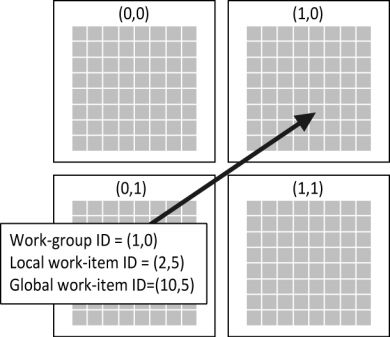
\includegraphics[width=0.50\textwidth]
	{pics/opencl-work.jpg}
	\caption{Work group dan work item pada OpenCL dan Vulkan .}
	\label{fig:work}
\end{figure}

Saat suatu proses berjalan pada device, dapat diambil ID dari work item atau work group yang menjalankan proses tersebut. Dengan demikian dapat diatur bagian data mana yang diproses oleh masing-masing ID. Misalnya dalam penjumlahan vektor, work item dengan ID i hanya memproses elemen ke i dari vektor-vektor yang dijumlahkan.